\documentclass[a4paper,12pt]{article}
%\documentclass[a4paper,10pt]{scrartcl}

\usepackage{scrextend}
\changefontsizes[14pt]{14pt}

\usepackage[T1]{fontenc}
\usepackage{lmodern}
\usepackage[utf8x]{inputenc}
\usepackage{graphicx}
\usepackage{tabularx}
\usepackage{multirow}
\usepackage{booktabs}
\usepackage{colortbl}
\usepackage[italian]{babel}
\usepackage[margin=2cm]{geometry}
\usepackage{color}
\definecolor{mygrey}{gray}{0.4}
\definecolor{light-blue}{rgb}{0.4,0.5,1}
\definecolor{light-cyan}{rgb}{0.4,0.6,1}
\usepackage{booktabs}

%Header and footer of pages
\usepackage{fancyhdr}
\pagestyle{fancy}
\lhead{\textcolor{mygrey}{Emanuele Uliana, Gabriele Rufolo, Walter Rubino}}
\rhead{\textcolor{mygrey}{Manuale d'uso}}

%Set paragraphs indentation to 0 points
\setlength{\parindent}{0pt}

%Sections and subsections' style
\usepackage{titlesec} 
\titleformat{\section} {\color{blue}\normalfont\sffamily\Large\bfseries} {\color{blue}\thesection}{20pt}{} 
\usepackage{titlesec}
\titleformat{\subsection} {\color{light-blue}\normalfont\sffamily\large\bfseries\itshape} {\color{light-blue}\thesubsection}{18pt}{} 
\titleformat{\subsubsection} {\color{light-cyan}\normalfont\sffamily\large\bfseries\itshape} {\color{light-cyan}\thesubsubsection}{14pt}{} 



%Document default font family
\renewcommand{\familydefault}{\sfdefault}
\renewcommand*\arraystretch{1.5}

\pdfinfo{%
  /Title    (SWIMv2 - Manuale d'uso)
  /Author  (Emanuele Uliana /and Gabriele Rufolo / and Walter Rubino)
  /Creator  (Emanuele Uliana /and Gabriele Rufolo / and Walter Rubino)
  /Producer (Emanuele Uliana /and Gabriele Rufolo / and Walter Rubino)
  /Subject  (Manuale d'uso)
  /Keywords ()

}

\begin{document}
\vspace*{\fill}
\begin{center}
{\fontsize{28}{10} \selectfont \textcolor{mygrey}{Progetto di Ingegneria del Software 2} \\[2\baselineskip]} {\fontsize{42}{10} \selectfont {\bfseries SWIMv2}} \\[4\baselineskip]

\includegraphics[scale=1]{wave-icon} \\[4\baselineskip]
{\fontsize{28}{10} \selectfont {\bfseries \textcolor{blue}{Manuale d'uso}} \\[2\baselineskip] A.A. 2012/2013}
\end{center}
\begin{flushleft}
{\fontsize{18}{10}
{\bfseries Autori}: \\ Emanuele Uliana (799256), Gabriele Rufolo (743695), Walter Rubino (742519) \\[1\baselineskip]
{\bfseries Docente}: \\ Prof.ssa Raffaela Mirandola
}
\end{flushleft}
\vspace*{\fill}
\begin{center}
Versione 1.0 del 24/1/2013 \\
\end{center}

\clearpage

	    \vspace*{\fill}
	\tableofcontents
	    \vspace*{\fill}

\clearpage

\section{Installazione}
Per installare correttamente il tutto si consiglia di leggere il manuale di installazione che si trova nella repo del progetto ``learning-to-swim'' nella sezione downloads.

\section{Precondizioni e Postcondizioni (con la gentile partecipazione di Carlo Ghezzi)}
Dopo aver completato l'installazione, le precondizioni fondamentali per un corretto comportamento del sistema sono:

\begin{itemize}
 \item Usare un browser aggiorato che supporti Javascript, Java e HTML 5
 \item Avere installato almeno il jre 1.6 o, in alternativa l'openjdk 1.6
 \item Avere attivi javascript e l'accettazione di cookie nel browser
 \item Non avere attive sul browser estensioni come NoScript che bloccano il caricamento dei Javascript
 \item E dulcis in fundo la principale precondizione:
 \begin{itemize}
  \item DO NOT USE INTERNET EXPLORER!
  \item YOU MUST NOT USE INTERNET EXPLORER!!
  \item THOU SHALT NOT USE INTERNET EXPLORER!!!
 \end{itemize}
 Seriously: it sucks, any version of it is an unpunished crime.
\end{itemize}
Dopo questo piccolo sfogo in lingua inglese (giusto perchè le parole suonano meglio e più solenni), vorrei ricordare a tutti coloro che hanno avuto il professor Carlo Ghezzi a Ingegneria del Software 1 (per chi non l'avesse avuto, niente paura: ripeterò le
sue parole), le sue parole a proposito del rapporto tra precondizioni e postcondizioni: \linebreak

``Se le precondizioni sono verificate, allora anche le postcondizioni devono esserlo, ma se le precondizioni non sono verificate, può anche cadere una bomba.'' 
\linebreak

- cit. Carlo Ghezzi


\vspace{0.5cm}
Di conseguenza, se usate il browser dell'azienda di Redmond, ... (no need to continue)

Se invece le precondizioni sono rispettate, la postcondizione è che il sistema farà correttamente ciò per cui è stato progettato; questo manuale d'uso (di un social network!) spiegherà dettagliatamente come
muovere i primi passi nel mondo di SWIMv2.

\pagebreak

\section{Funzionalità accessibili a un ospite}
Dalla Homepage http://127.0.0.1:8080/Directory-di-installazione/index.jsp un ospite può effettuare la ricerca di utenti, la registrazione ed il login.

\subsection{Ricerca di utenti}
Si noti che la procedura di ricerca è identica per utenti registrati e amministratori, con la differenza che gli ospiti non possono visualizzare i dettagli del profilo degli utenti
trovati.
\linebreak
La ricerca può essere effettuata per nome e cognome, oppure per abilità.

\subsubsection{Ricerca per nome e cognome}
L'utente deve obbligatoriamente scrivere qualcosa in almeno uno dei due campi (un Javascript controlla ciò, e in caso di form completamente vuota, non permette l'invio dei dati alla
servlet), e i risultati visualizzati sono i nomi e cognomi di tutti gli utenti che hanno almeno uno dei due campi (nome e cognome) uguale ai corrispondenti dati in input, ad esempio:
\\
\vspace{0.1cm}
\\
Se viene cercato Emanuele Uliana, viene ritornato Emanuele Uliana, ma anche Emanuele Tizio e Caio Uliana vengono visualizzati (dando per scontato che i 3 utenti siano nel database).
\\
\vspace{0.1cm}
\\
Se invece non esistono utenti compatibili con i dati in ingresso, verrà visualizzato un apposito messaggio di ricerca senza risultati.

\subsubsection{Ricerca per abilita'}
Ancora una volta non è possibile effettuare una ricerca vuota, e in questo caso, il campo da riempire è solo 1 e lì va inserito il nome dell'abilità della quale si è interessati a
trovare tutti gli utenti che la possiedono. I risultati visualizzati saranno tutti e soli gli utenti che possiedono tale abilità, oppure un messaggio che indica l'assenza dei medesimi.

\subsection{Registrazione}
La procedura di registrazione consiste nel riempire tutti i campi dell'apposita form con i seguenti vincoli:

\begin{itemize}
 \item Tutti i campi devono essere riempiti: in caso contrario i dati non verranno nemmeno inviati alla servlet corrispondente e verra' visualizzato un popup di errore.
 \item I campi ``password'' e ``conferma password'' devono necessariamente contenere la stessa stringa (non vuota): in caso contrario valgono le considerazioni del punto precedente.
 \item La mail deve essere un'espressione regolare di questo tipo: \\
 
 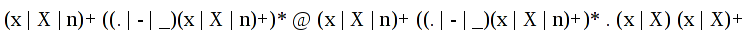
\includegraphics[scale=0.6]{email} 
 
 dove:
 
 \begin{itemize}
  \item Le parentesi ( e ) hanno un ruolo ovvio.
  \item il simbolo ``pipe'' | ha la funzione di OR logico.
  \item il simbolo * rappresenta la stella di Kleene.
  \item il simbolo + rappresenta l'operatore croce.
  \item i simboli punto, trattino, underscore e chiocciola sono dei caratteri che possono essere contenuti nella stringa, compatibilmente con le regole dell'espressione regolare.
  \item i simboli x, X, n indicano rispettivamente una lettera minuscola dell'alfabeto inglese, una lettera maiuscola dell'alfabeto inglese e una cifra da 0 a 9.
 \end{itemize}

 
 Spero abbiate studiato Linguaggi Formali e Compilatori... In ogni caso, se l'email non è di quel tipo, la registrazione fallirà e seguirà un redirect alla homepage.
 \item L'email deve esistere: nonostante per ovvi motivi ciò non sia verificabile, la procedura di registrazione inserisce l'utente nel database come ``utente non confermato'' e
 spedisce all'indirizzo email fornito una mail contenente un link che dovrà essere necessariamente visitato per confermare il proprio account e poter così effettuare il login.
\end{itemize}

In caso la procedura vada a buon fine, e dopo aver confermato il proprio account, si verrà reindirizzati alla homepage con un messaggio informativo. A questo punto è possibile
effettuare correttamente la procedura di login.

\subsection{Login}
La procedura di login consiste nel riempire i campi ``email'' e ``password'' dell'apposita form con i seguenti vincoli:

\begin{itemize}
 \item I due campi devono essere riempiti: in caso contrario i dati non verranno nemmeno inviati alla servlet corrispondente e verra' visualizzato un popup di errore.
 \item I dati inseriti devono essere corretti: in caso contrario il login fallira' e si verrà reindirizzati alla homepage con un messaggio di errore.
\end{itemize}

In caso la procedura vada a buon fine, comparirà la pagina personale con tutte le funzionalità accessibili a un utente registrato e loggato.

\section{Funzionalita' accessibili ad un utente registrato e loggato}

Dalla pagina di profilo l'utente loggato può accedere alle funzionalità di gestione amicizie, gestione messaggi (che include la gestione feedback), gestione profilo e ricerca utenti.

\subsection{Gestione amicizie}

\subsection{Gestione messaggi}

\subsubsection{Gestione feedback}

\subsection{Gestione profilo}

\subsubsection{Gestione Abilita'}

\subsection{Ricerca utenti}
Non è diversa dalla ricerca accessibile agli ospiti, con la differenza che, se effettuata da utenti registrati, permette di cliccare sui risultati per accedere alla pagina del profilo
dell'utente selezionato in modalità di visitatore (cioè non vengono visualizzate alcune funzionalità accessibili da quell'utente quando lui è loggato).

\section{Funzionalità accessibili ad un amministratore}

Un amministratore (di default l'unico amministratore che i tester possono usare è The King, che ha come email theking@emailtemporanea.net e come password skyrimisevil) può accedere a
tutte le funzionalità già descritte nella sezione degli utenti normali e in più può gestire il set di abilità di sistema, aggiungendone su richiesta.

\subsection{Gestione set di abilità di sistema}

\end{document}